% Chapter 4
\chapter{Transmission Expansion Planning by Quantum Annealing} % Main chapter title
\label{Chapter4} % For referencing the chapter elsewhere, use \ref{Chapter1} 
\section{Statement of the problem}
\begin{wrapfigure}{l}{0.4\textwidth}
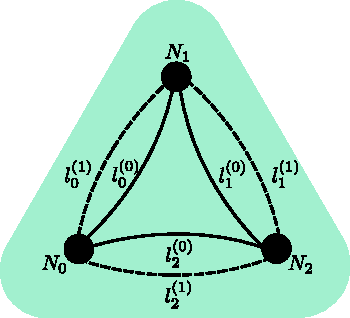
\includegraphics[scale=0.9]{Figures/3Node_Layer 1.pdf} 
\caption{An example considering a three node transmission expansion planning (TEP) problem with three candidate lines. Solid lines represent existing lines (super-index $(0)$) and dash lines are the candidate lines (super-index $(1)$).}
\label{fig:3node}
\end{wrapfigure}
\textit{Transmission expansion planning} (TEP) consist in determining where, when and what to build to the existing network to fulfill the energy demand in a future scenario. 
More precisely, it determines where and when to build new transmission lines between nodes. There are other components of a network that can be built to satisfy future energy demand, carbon emissions or other targets. As an example, capacity expansion planning decides where, when and what type of generator to build -- wind turbine, heat pump, solar panels ... -- to an existing network so that fulfill energy demands in a future scenario. Often these problems of improving the existing network to fulfill future targets are taken into account together under the name transmission expansion planning but in this case we are considering just transmission lines.\par
\begin{wraptable}{r}{0.4\textwidth}
\centering
\begin{tabular}{cc} \\\toprule 
 \textbf{Symbol} & \textbf{Description} \\\midrule
 $\mathcal{N}$ & Nodes  \\\midrule
 $\mathcal{L}^{(0)}$ & Existing transmission lines  \\\midrule
  $\mathcal{L}^{(1)}$ & Candidate transmission lines \\\midrule
 $\mathcal{D}_{i}$ & Demand of node $i$. \\\midrule
 $\mathcal{C}_{i}$ & Investment cost of line $i$ \\\bottomrule 
\end{tabular}
\caption{Nomenclature.}
\label{table:TEPNomenclature}
\end{wraptable}
We start by considering an small network of three nodes $N_{i}\in \mathcal{N}$ with 3 existing lines $l_{i}^{(0)}\in \mathcal{L}^{(0)}$ and 3 candidate lines $l_{i}^{(1)}\in \mathcal{L}^{(1)}$. Our target is going to be a given energy demand in a future scenario. The nodes can be though as towns whose energy demand has to be fulfilled and the lines allow the network to transmit energy between nodes so that if some node is producing more energy than its demand, then this excess of energy can be transmitted to other node in the network.
%%%%%%%%%%
We start by considering an small network of three nodes $N_{i}\in \mathcal{N}$ with 3 existing lines $l_{i}^{(0)}\in \mathcal{L}^{(0)}$ and 3 candidate lines $l_{i}^{(1)}\in \mathcal{L}^{(1)}$. Our target is going to be a given energy demand in a future scenario. The nodes can be though as towns whose energy demand has to be fulfilled and the lines allow the network to transmit energy between nodes so that if some node is producing more energy than its demand, then this excess of energy can be transmitted to other node in the network.
We start by considering an small network of three nodes $N_{i}\in \mathcal{N}$ with 3 existing lines $l_{i}^{(0)}\in \mathcal{L}^{(0)}$ and 3 candidate lines $l_{i}^{(1)}\in \mathcal{L}^{(1)}$. Our target is going to be a given energy demand in a future scenario. The nodes can be though as towns whose energy demand has to be fulfilled and the lines allow the network to transmit energy between nodes so that if some node is producing more energy than its demand, then this excess of energy can be transmitted to other node in the network. We start by considering an small network of three nodes $N_{i}\in \mathcal{N}$ with 3 existing lines $l_{i}^{(0)}\in \mathcal{L}^{(0)}$ and 3 candidate lines $l_{i}^{(1)}\in \mathcal{L}^{(1)}$.
Our target is going to be a given energy demand in a future scenario. The nodes can be though as towns whose energy demand has to be fulfilled and the lines allow the network to transmit energy between nodes so that if some node is producing more energy than its demand, then this excess of energy can be transmitted to other node in the network.
We start by considering an small network of three nodes $N_{i}\in \mathcal{N}$ with 3 existing lines $l_{i}^{(0)}\in \mathcal{L}^{(0)}$ and 3 candidate lines $l_{i}^{(1)}\in \mathcal{L}^{(1)}$. Our target is going to be a given energy demand in a future scenario. The nodes can be though as towns whose energy demand has to be fulfilled and the lines allow the network to transmit energy between nodes so that if some node is producing more energy than its demand, then this excess of energy can be transmitted to other node in the network.
\section{Formulation of QUBO}
\section{Running QUBO problem on D-WAVE's annealer}

